\pdfoutput=1

\documentclass[prd,amsmath,amssymb,floatfix,nofootinbib,superscriptaddress, twocolumn]{revtex4}

\usepackage{bm}
\usepackage{amsmath}
\usepackage{epsfig}
\usepackage{color}
\usepackage{natbib}
\usepackage{graphicx}
\usepackage{enumerate}
\usepackage{natbib}
%\usepackage[hypertex]{hyperref}
\usepackage{ifthen}

\def\eprinttmp@#1arXiv:#2 [#3]#4@{
\ifthenelse{\equal{#3}{x}}{\href{http://arxiv.org/abs/#1}{#1}}{\href{http://arxiv.org/abs/#2}{arXiv:#2} [#3]}}

\providecommand{\eprint}[1]{\eprinttmp@#1arXiv: [x]@}
\newcommand{\adsurl}[1]{\href{#1}{ADS}}
%\newcommand{\bibinfo}[2]{\ifthenelse{\equal{#1}{isbn}}{
%\href{http://cosmologist.info/ISBN/#2}{#2}}{#2}}

\newcommand{\edth}{\;\raise1.0pt\hbox{$'$}\hskip-6pt\partial}
\newcommand{\spin}[1]{\,{}_{#1}^{\vphantom{m}}}

\newcommand{\ylm}[2]{Y_{#1 #2}}
\newcommand{\yslm}[3]{\spin{#1} Y_{#2 #3}}

\newcommand{\rlm}[2]{R_{#1 #2}}
\newcommand{\slm}[4]{\spin{#2} {#1}_{#3 #4}}

\def\pos{\hat{n}}

\def\be{\begin{equation}}
\def\ee{\end{equation}}
\def\ba{\begin{eqnarray}}
\def\ea{\end{eqnarray}}

\def\nn{\nonumber}

\newcommand{\clo}{{\cal O}}
\newcommand{\wt}{{\cal G}}

\newcommand{\dmh}[1]{\textcolor{blue}{(DMH: #1)}}

\newcommand{\threej}[6]{\left(
                           \begin{array}{ccc}
        \! #1\! & #2\!  & #3\!  \\
        \! #4\! & #5\!  & #6\!
                           \end{array}
                   \right)}

\newcommand{\sixj}[6]{\left\{
                           \begin{array}{ccc}
        \! #1\! & #2\!  & #3\!  \\
        \! #4\! & #5\!  & #6\!
                           \end{array}
                   \right\}}

 \newcommand{\vect}[1]{\bm{#1}}

\begin{document}

\title{Spherical Harmonic Transform Notes}

\begin{abstract}
\end{abstract}
\maketitle

\section{Spherical harmonics}
\label{sec:app:spht:ylm}
%
A scalar field $f(\pos)$ on the sphere can be represented 
using spherical harmonic coefficients $a_{lm}$ given by
\ba
a_{lm} &=& \int \ylm{l}{m}^*(\pos) f(\pos) \label{eqn:alm} \\
f(\pos) &=& \sum_{lm} a_{lm} \ylm{l}{m}(\pos) \label{eqn:fofn}.
\ea 
The harmonics $\ylm{l}{m}$ are eigenfunctions of the
Laplacian on the sphere, and the decomposition above
is analogous to a Fourier expansion on the plane.

The harmonics obey the relation 
$\ylm{l}{m} = (-1)^m \ylm{l}{(-m)}^*$
and so for $f(\pos)$ which is real
we have $a_{lm} = (-1)^m a_{l(-m)}$.
In this case, we can alternatively
decompose $f(\pos)$ using the real
spherical harmonics $R_{lm}$, defined by 
\begin{eqnarray} \label{E:realcomplex}
     R_{lm} = \left\{\begin{array}{ll}
     \frac{1}{\sqrt{2}}(\ylm{l}{m}+\ylm{l}{m}^*)&\mbox{if $m>0$} \\
     Y_{l0}&\mbox{if $m=0$} \\
     \frac{(-1)^m}{{\rm i}\sqrt{2}}(\ylm{l}{m}^*-\ylm{l}{m})&\mbox{if $m<0$}\,;
     \end{array} \right.
\end{eqnarray}
The corresponding decomposition of $f(\pos)$ is then
\ba
r_{lm} &=& \int \rlm{l}{m}(\pos) f(\pos) \label{eqn:rlm} \\
f(\pos) &=& \sum_{lm} r_{lm} \rlm{l}{m}(\pos).
\label{eqn:forfn}
\ea
This representation is often simpler to work with on a computer,
as it means that the coefficients and their covariance matrices are real.

\section{Spin-s Spherical harmonics}
\label{sec:app:spht:yslm}
Complex quantities on the sphere are often spin fields. 
Under rotation of the coordinate system by an angle $\alpha$, the representation of these fields at the 
origin of the rotation must acquire an opposing phase of $e^{-i s \alpha}$ to remain physically consistent, where
$s$ is referred to as the spin, or spin-weight.
Both the (Q,U) representation of polarization (with $s=2$) as well as lensing deflection vectors (with $s=1$) are spin fields. 
To work with such spin-$s$ quantities it is useful to represent them in a basis which 
absorbs this coordinate-dependent phase. Such a basis may be constructed from the 
standard (spin-0) spherical harmonics by the operation of spin raising and lowering operators. 
On the plane these operators are intuitively given by
%
\begin{equation}
\edth_{\pm} = \left[ \frac{\partial}{\partial x} \pm i \frac{\partial}{\partial y} \right].
\end{equation}
%
%Operating on a some spin field, these operators have the property of raising or lowering its spin weight by one.
On the sphere, the situation is complicated by the connection which mixes the coordinate basis 
vectors under differentiation. The spin operators become \cite{NewPenNotes}
%
\begin{equation}
\edth_{\pm} = -(\sin \theta)^{\pm s} \left[ \frac{\partial}{\partial \theta} \pm \frac{i}{\sin \theta}\frac{\partial}{\partial \phi} \right] (\sin \theta)^{\mp s}.
\end{equation}
%
We can then define the spin-$s$ spherical harmonics as a natural extension of the standard spherical harmonics.
Using the convention
%
\begin{eqnarray}
{}_{s} Y_{lm} = 
\left\{\begin{array}{ll}
     \sqrt{\frac{ (l - s)! }{(l + s)!}} \edth_{+}^{s} \ylm{l}{m} & (0 \le s \le l) \\
     \sqrt{\frac{ (l+ s)! }{(l  - s)!}} (-1)^{s} \edth_{-}^{-s}  \ylm{l}{m}  & (-l \le s \le 0) \\
     0 & (l < |s|).
     \end{array} \right.
\end{eqnarray}
%
The normalization factor ensures that the magnitude $| {}_s Y_{lm} |^2$ 
integrates to unity over the sphere. A complex spin-$s$ quantity ${}_s f(\pos)=[\alpha_1 + i
\alpha_2](\pos)$ 
may then be decomposed into harmonic coefficients ${}_s v_{lm}$ as
%
\begin{equation}
{}_s v_{lm} = \int {}_s f(\pos) \yslm{s}{l}{m}^*(\pos) .
\label{eqn:spht_transform}
\end{equation}
%
The spin-$s$ harmonics obey the parity relation
%
\begin{equation}
\yslm{s}{l}{m}( \pi - \theta, \phi + \pi) = (-1)^{l} \yslm{-s}{l}{m}(\theta,\phi).
\label{eqn:parity}
\end{equation}
%
This often makes it useful, instead of ${}_s v_{lm}$ to work with the 
gradient/curl modes defined by
%
\begin{equation}
\int \yslm{\pm |s|}{l}{m}^*(\pos) [\alpha_1 \pm i
\alpha_2](\pos) = - (\pm)^{|s|} [G_{lm} \pm iC_{lm}].
%\int d\Omega \yslm{\pm s}{l}{m} [\alpha_1 \pm i \alpha_2] = - (\pm)^{s} [G_{lm} \pm i C_{lm}]
\end{equation}
In the spin-2 case G/C are usually referred to as E/B modes.
The overall negative sign is designed for consistency with 
\cite{Zaldarriaga:1996xe,Gorski:2004by}
and the $(\pm)^{|s|}$ ensures that the gradient 
of a scalar function (a spin-1 quantity) is entirely G-mode.
By construction, the $G$ and $C$ modes are parity eigenstates. 
The $G_{lm}$ acquire a sign of $(-1)^{l}$ and the $C_{lm}$ 
acquire a sign of $(-1)^{l+1}$ under a parity transformation.
%
In terms of the fundamental transform of 
Eq.~\eqref{eqn:spht_transform}
we have
%
\begin{align}
G_{lm} &= -\frac{1}{2}  [ {}_{|s|} v_{lm} + (-1)^{m} {}_{|s|} v^*_{l(-m)} ] 
\\ C_{lm} &= -\frac{1}{2i} [ {}_{|s|} v_{lm} - (-1)^{m} {}_{|s|} v^*_{l(-m)} ].
\end{align}
%

\subsection{Recursion relations}

%
\begin{figure}[!ht]
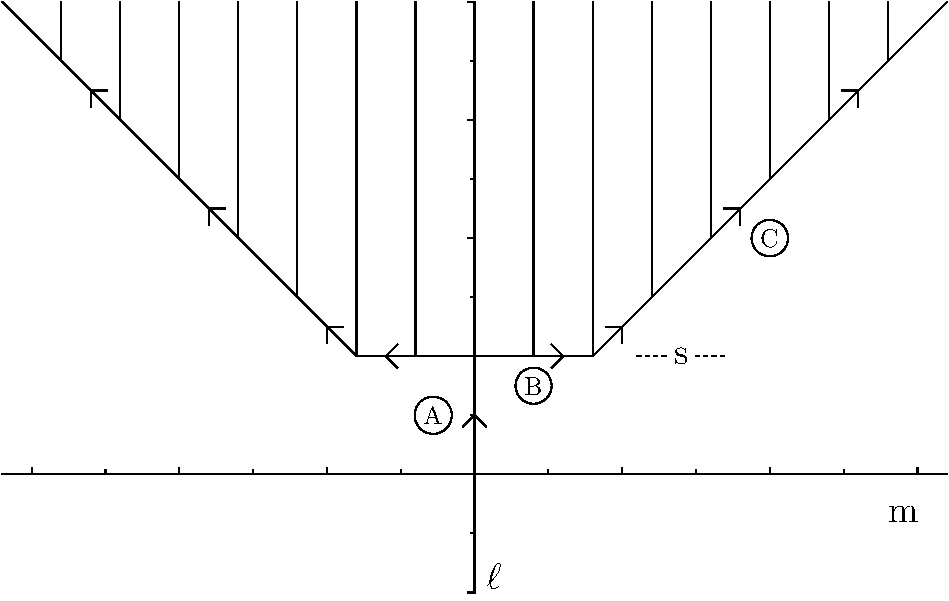
\includegraphics[width=\columnwidth]{rec_graph.pdf}
\caption{Diagram illustrating the recursions in the $(l,m)$ plane to determine ${}_{s} \lambda_{l m}$.}
\label{fig:recursion_minimal}
\end{figure}
%
The spin-s spherical harmonics are separable in $\theta$, $\phi$, and can be written as
%
\begin{equation}
\yslm{s}{l}{m}(\theta,\phi) = {}_{s} \lambda_{lm} (\theta) e^{im\phi}.
\end{equation}
%
The ${}_s \lambda_{lm}$ are real, and the only complex contribution
to $\yslm{s}{l}{m}$ comes from $e^{im\phi}$.

To calculate the ${}_s \lambda_{lm}$ the following 
recursion relation is useful \cite{Lewis:2001hp}:
%
\begin{multline}
{}_{s} \lambda_{lm} = 
\Bigg[ \left( \cos(\theta) + \frac{s m}{l(l-1)} \right)  {}_s \lambda_{(l-1)\ m} \\
- {}_s \lambda_{(l-2)\ m}/ r_{s (l-1) m} \Bigg]  r_{s l m},
\label{eqn:rec_l}
\end{multline}
%
where 
%
\begin{equation}
r_{slm} = \sqrt{\frac{l^2 (4l^2 - 1)}{ (l^2 - m^2)(l^2 - s^2) }}.
\end{equation}
%
To determine starting points for the recursion we can use an explicit formula for ${}_s \lambda_{l m}$ from Goldberg~et.~al. \cite{goldberg:2155}: \footnote{Note that we use the Condon-Shortley phase convention, which differs from their definition of the harmonics by a factor of $(-1)^{m}$.}
\begin{multline}
{}_{s} \lambda_{l m} (\theta) 
= \sqrt{ \frac{ (l+m)! (l-m)!}{(l+s)!(l-s)!} \frac{(2l+1)}{4\pi} }
\sin^{2l}\left(\frac{\theta}{2}\right) 
\\ \times\sum_{r} {l-s \choose r} 
{l+s \choose r+s-m}
\\ \times (-1)^{l+m-r-s}
\cot^{2r+s-m}\left(\frac{\theta}{2}\right).
\end{multline}
%
This leads to three relations which can be used to move through the $(l,m,s)$ space:
%
\begin{align} 
{}_s \lambda_{s 0}(\theta) &= 
+\sqrt{\frac{(2s+1)}{2s}} \sin(\theta) {}_{(s-1)} \lambda_{(s-1) 0} \tag{A} 
\\ {}_s \lambda_{s (\pm |m|)}(\theta) &= 
-\sqrt{ \frac{(s-|m|+1)}{s+|m|} } \tan^{\pm 1}\left( \frac{\theta}{2} \right) {}_{s} \lambda_{s (\pm (|m|-1))} \tag{B} 
\\ {}_s \lambda_{l (\pm l)} &= 
\mp \sqrt{ \frac{l(2l+1)}{2(l+s)(l-s)} } \sin(\theta) {}_{s} \lambda_{(l-1)(\pm (l - 1))} \tag{C}.
\label{eqn:rec_sm}
\end{align}
%
Fig.~\ref{fig:recursion_minimal} illustrates the use of
these relations to move into a starting location for the $l$
recursion of Eq.~\eqref{eqn:rec_l} from the origin at
$\yslm{0}{0}{0} = 1/\sqrt{4\pi}$. 


\bibliography{shts}

\appendix

\end{document}